\clearpage{\pagestyle{empty}\cleardoublepage}
\chapter{Contesto del progetto}
\textbf{Pathadora} è un sistema di raccomandazione progettato per suggerire agli studenti le facoltà e i corsi più idonei per loro sulla base delle informazioni specificate, sia personali che relative a eventuali disabilità possedute. 

Pathadora può essere suddiviso in due sottosistemi: 
\begin{itemize}
\item \textbf{Pathadora Web App}, permette all'utente di interfacciarsi con il sistema di raccomandazione creando un proprio profilo per poi sottomere richieste per ottenere risultati su facoltà, corsi e risorse didattiche suggerite. Permette inoltre la registrazione di profili per docenti, i quali possono caricare le risorse didattiche relative ai propri corsi per cui, quando possibile, verranno generati metadati relativi all'accessibilità del contenuto; queste verranno poi utilizzati dal sistema di raccomandazione per determinare se suggerire o meno la risorsa associata a utenti con determinate disabilità.
\item \textbf{Pathadora Recommender}, che memorizza le entità del dominio in un'ontologia del web semantico (\textit{Pathadora Ontology}) e produrrà i risultati relative a facoltà, corsi e risorse suggeriti utilizzando regole SWRL e SPARQL (\textit{Pathadora Rule Model}). Le operazioni vengono eseguite a seguito delle richieste HTTP ricevute dalla web app, intercettate mediante un server back-end (\textit{Pathadora Engine}).

Per permettere le interrogazioni su una grande quantità di dati è stato progettato un knowledge graph mediante la piattaforma \textbf{Stardog}. Un knowledge graph consiste nell'applicazione del modello descritto dall'ontologia su un insieme di istanze, \textit{individual}, collegati tra loro mediante relazioni.
\end{itemize}

\begin{figure}[H]
\centering
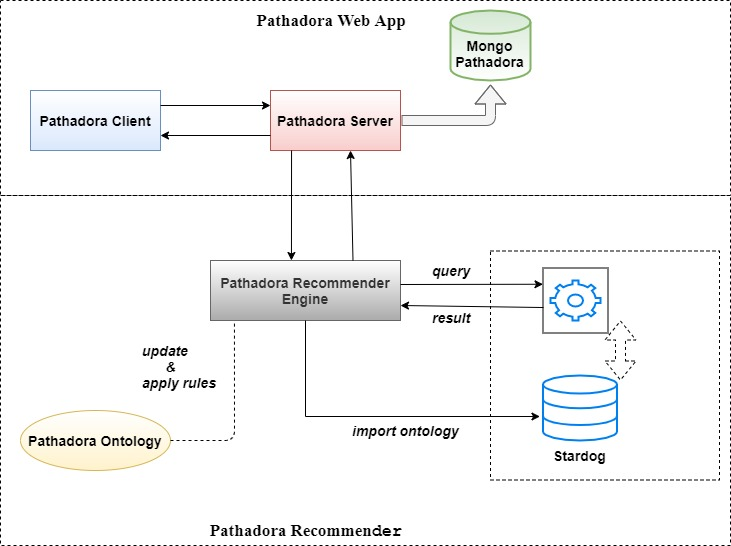
\includegraphics[scale=0.4]{res/pathadora-arch.jpg}
\caption{Architettura di Pathadora}
\label{fig:pathadora-arch}
\end{figure}

\begin{figure}[H]
\centering
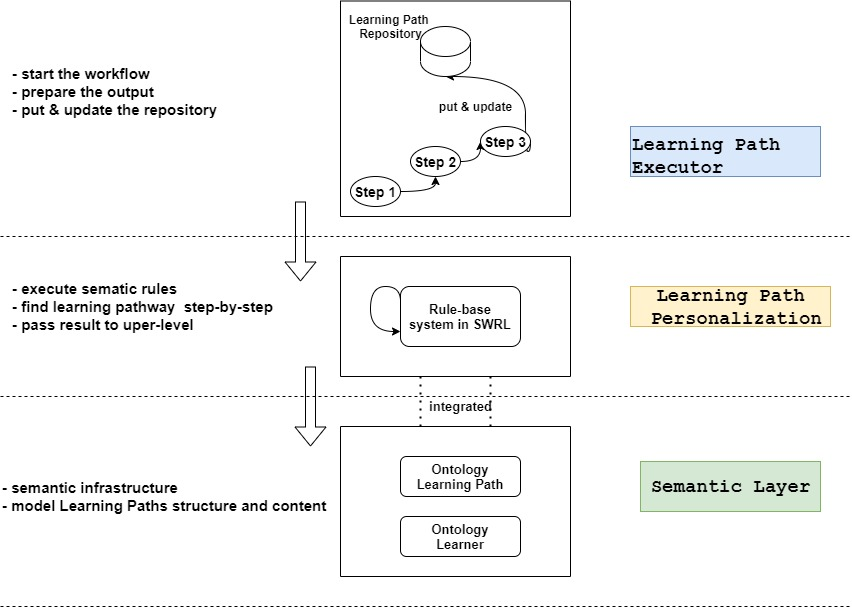
\includegraphics[scale=0.4]{res/diag-layers.jpg}
\caption{Workflow del sistema di raccomandazione}
\label{fig:diag-layers}
\end{figure}

\begin{figure}[H]
\centering
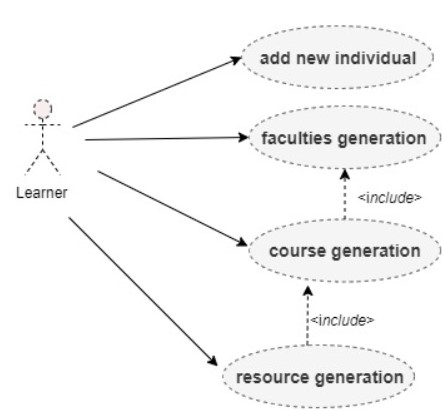
\includegraphics[scale=0.4]{res/pathadora-engine.jpg}
\caption{Casi d'uso sul Pathadora Recommender Engine}
\label{fig:pathadora-engine}
\end{figure}

\subsection{Richieste}
L'interfaccia web permette l'invio di richieste da sottomettere al Pathadora Engine attraverso appositi form.

\subsubsection{Inserimento}
La prima tipologia di richiesta da gestire è l’inserimento di nuove istanze nell'ontologia. In questa richiesta dovranno essere specificate tutte le informazioni che serviranno all’engine per aggiornare il knowledge graph. La richiesta potrebbe dichiarare relazioni tra elementi che non sono presenti e in tal caso, l’engine prima creerà questi elementi per poi definire la relazione tra
loro. Nel caso della richiesta di inserimento tutti gli elementi verranno aggiunti nell’ontologia, indipendentemente se esistono, se rispettano il formato giusto oppure se le relazioni sono semanticamente corrette.

\paragraph{Inserimento learner}
Alla registrazione di uno studente corrisponderà l'inserimento di un individual Learner nell'ontologia, le cui proprietà verranno utilizzate dal sistema per suggerire facoltà, corsi e risorse allo studente.

Le informazioni inserite riguardano le lingue conosciute, i titoli di laurea corrente e futuro, le passioni per determinati settori, gli obiettivi dello studente e il possedimento di determinate disabilità con relativi livelli associati.

\paragraph{Inserimento corsi}
Un docente registrato può personalizzare il suo profilo modificando le informazioni associate ai corsi di cui è titolare. I corsi inseriti saranno visualizzablii dagli studenti in una finestra dedicata.

Le informazioni associate al corso riguardano la lingua, il semestre di appartenenza, i CFU, l'anno, la tipologia (triennale, magistrale, dottorato), l'area scientifica di appartenenza e l'obbligatorietà del corso.

\paragraph{Inserimento risorse}
I docenti possono aggiungere risorse didattiche ai corsi a cui sono associati, descrivendoli con informazioni relative alla loro accessibilità.

 Le informazioni sono relative al tipo di adattamento, al grado di trasformazione applicabile su determinati elementi del contenuto (dimensione del testo), alla modalità di accesso e al tipo di risorsa. Verranno inoltre generati automaticamente indicatori numerici relativi al grado di leggibilità del testo contenuto in una risorsa, del rapporto di contrasto tra il colore del testo contenuto nelle immagini di un documento e relativo colore di sfondo, e della dimensione dei caratteri minima presente nel documento.

Le risorse potranno essere consultabili dagli studenti nella schermata dedicata ai corsi.

\subsubsection{Generazione di dipartimenti e facoltà}
A seguito della registrazione, lo studente può richiedere la generazione dei dipartimenti e delle facoltà suggerite, specificando il tipo di laurea (triennale, magistrale, dottorato) a cui fare riferimento. La generazione terrà conto delle informazioni dichiarate dallo studente durante la registrazione.

\begin{figure}[H]
\centering
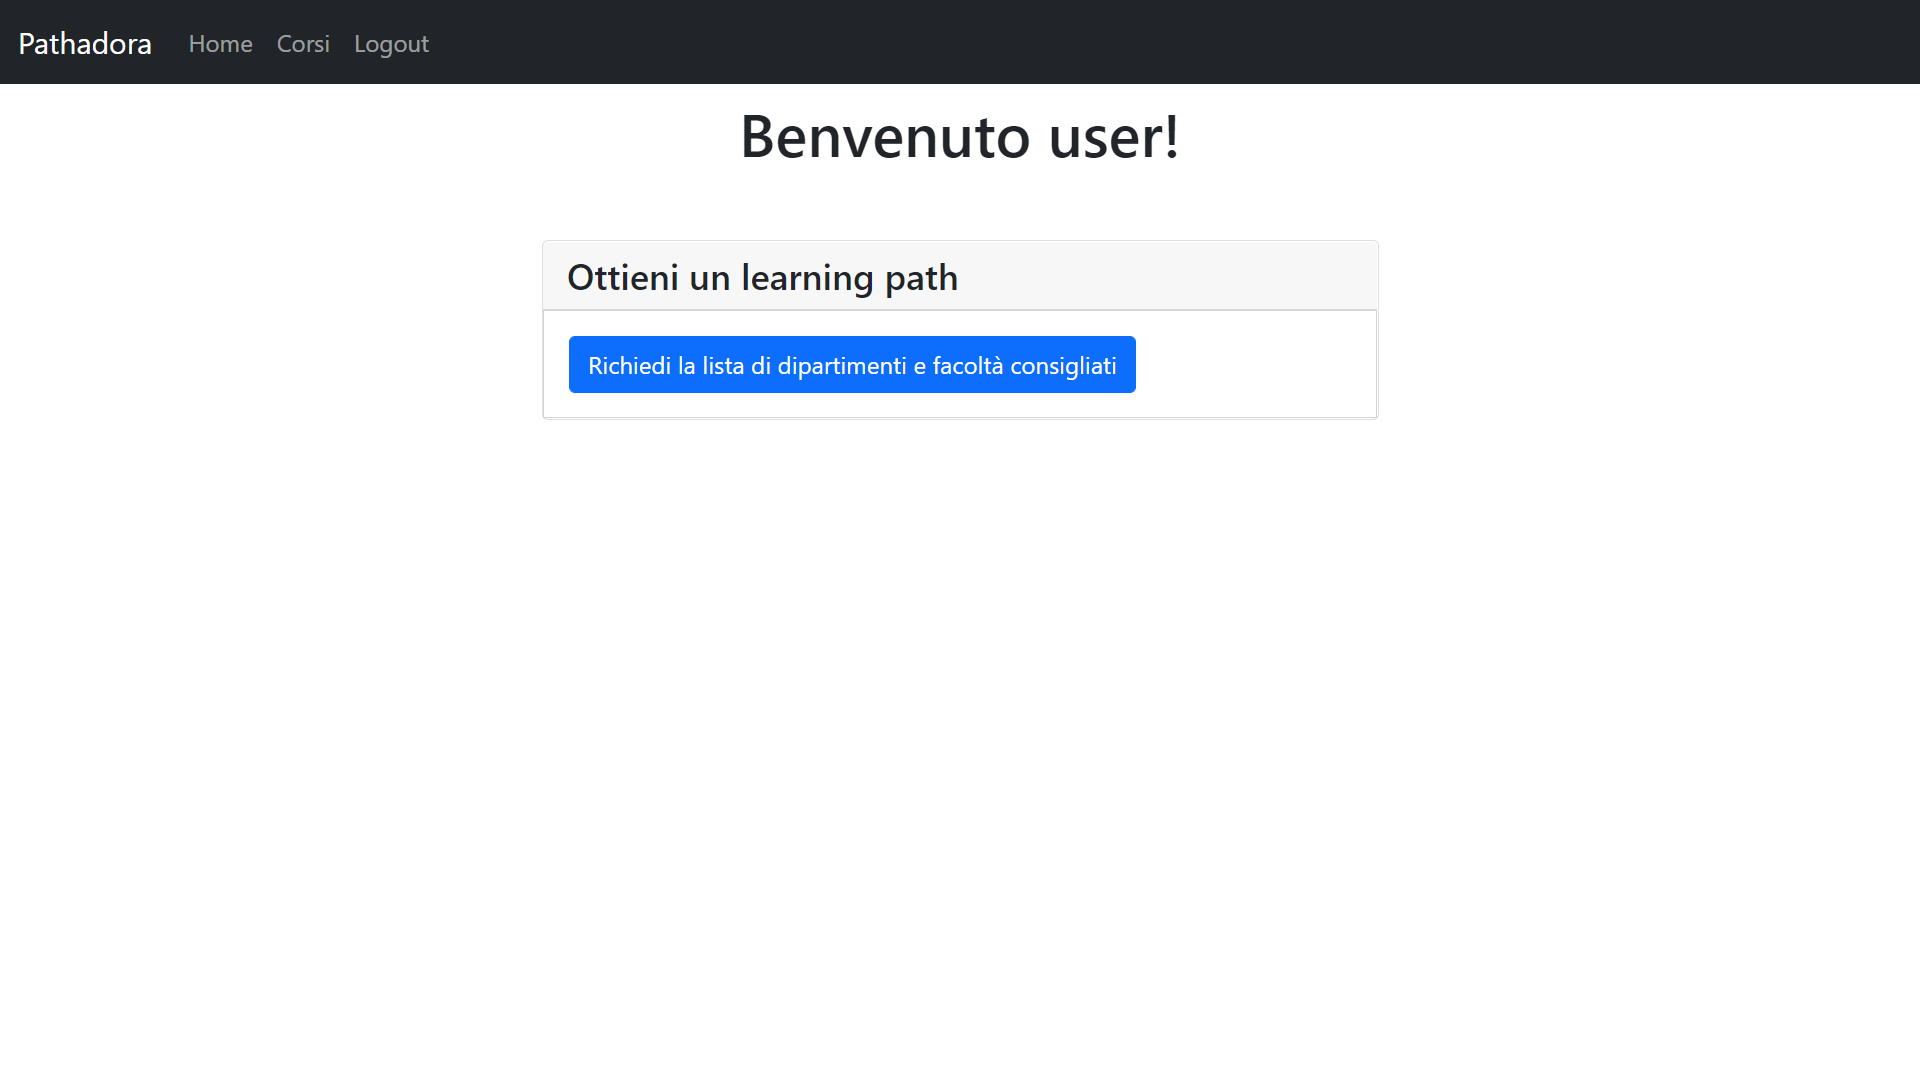
\includegraphics[scale=0.4]{res/faculties-generation.png}
\caption{Form di richiesta dipartimenti e facoltà suggeriti}
\label{fig:faculties-generation}
\end{figure}

\subsubsection{Generazione di corsi}
Una volta generate le facoltà, lo studente può richiedere la generazione dei corsi suggeriti selezionando la facoltà e l'anno preferiti. 
Una volta ricevuto tale scelta, il sistema inizializzerà il knowledge graph e lo interrogherà parametrizzando la query con le informazioni dello studente.

\begin{figure}[H]
\centering
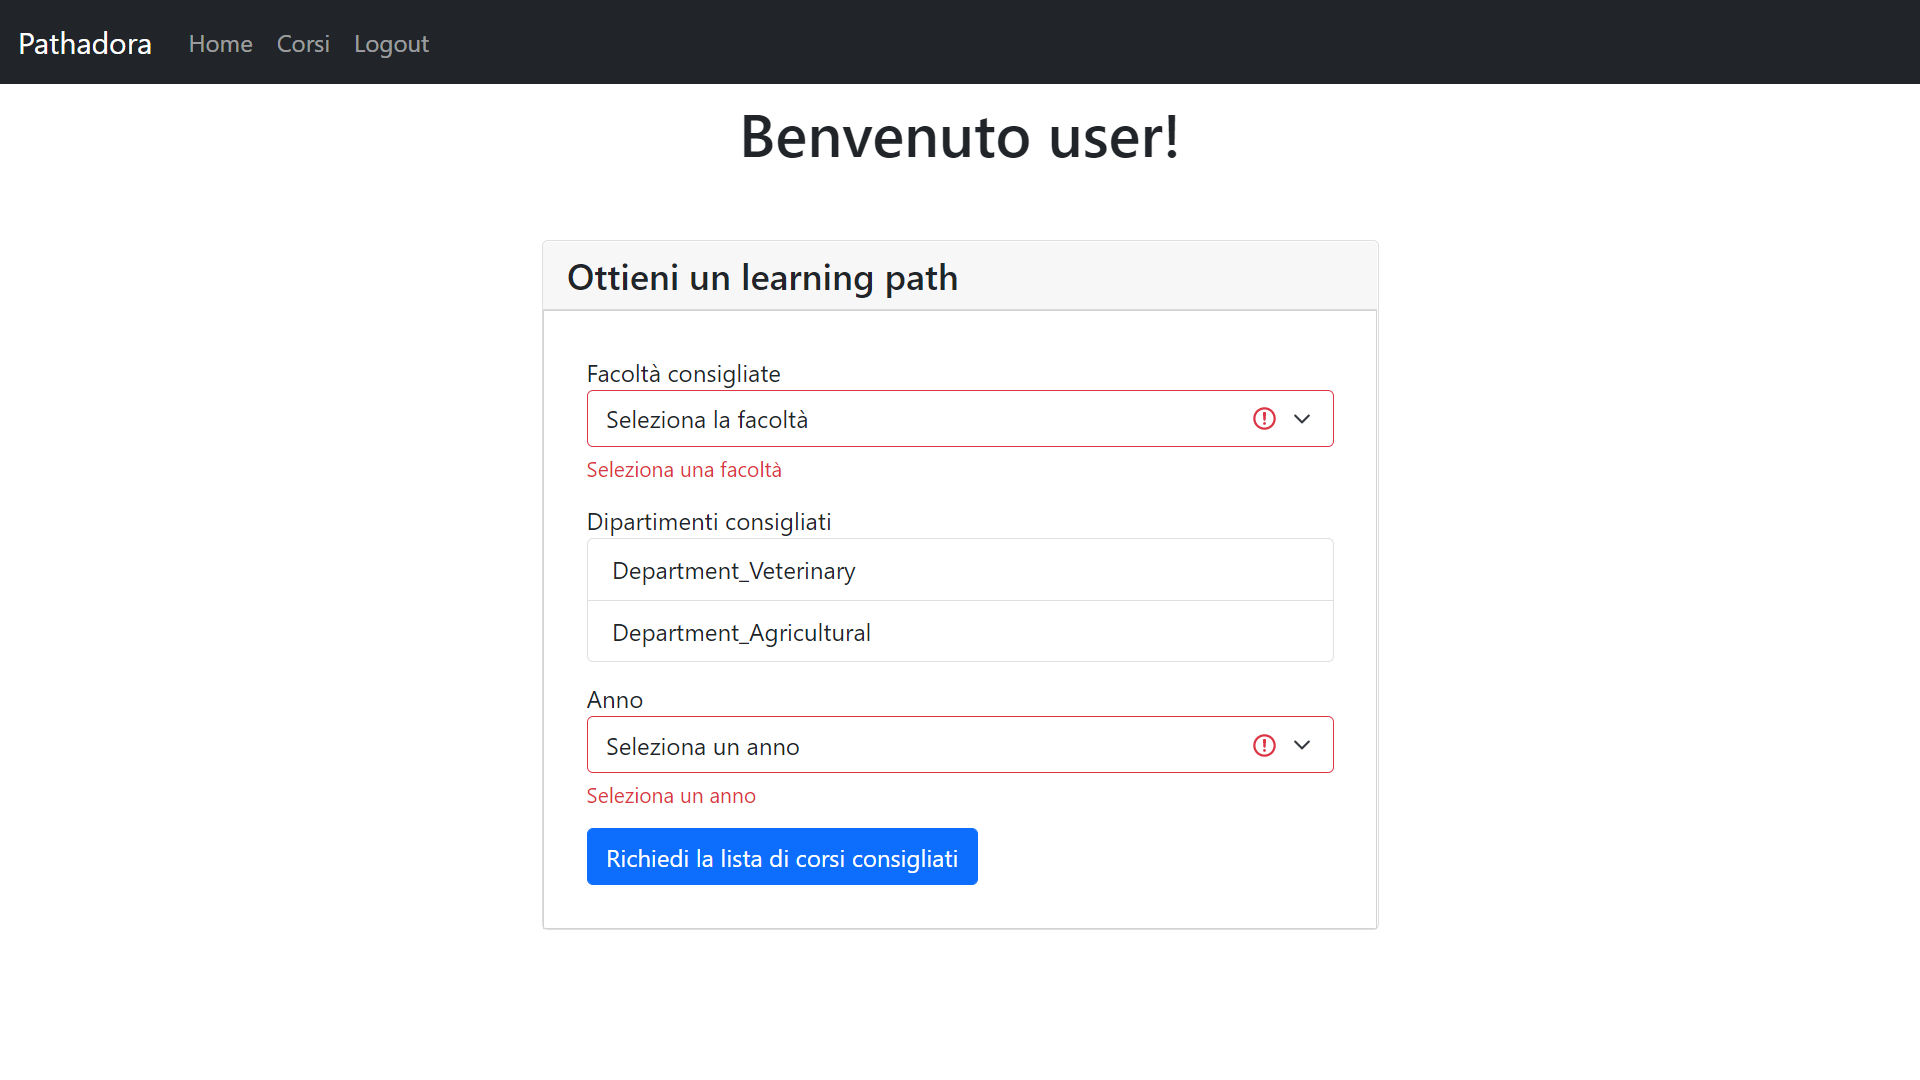
\includegraphics[scale=0.4]{res/courses-generation.png}
\caption{Form di richiesta corsi suggeriti}
\label{fig:courses-generation}
\end{figure}

\subsubsection{Generazione di risorse}
L'ultima richiesta da gestire consiste nella raccomandazione delle risorse relative a un corso specifico tra quelli suggeriti, risultati della richiesta precedente.
La raccomandazione terrà conto delle disabilità dello studente per determinare le risorse da raccomandare allo studente, a cui possono essere associate informazioni relative all'accessibilità come il grado di leggibilità del testo e la dimensione minima del font di un documento.

\begin{figure}[H]
\centering
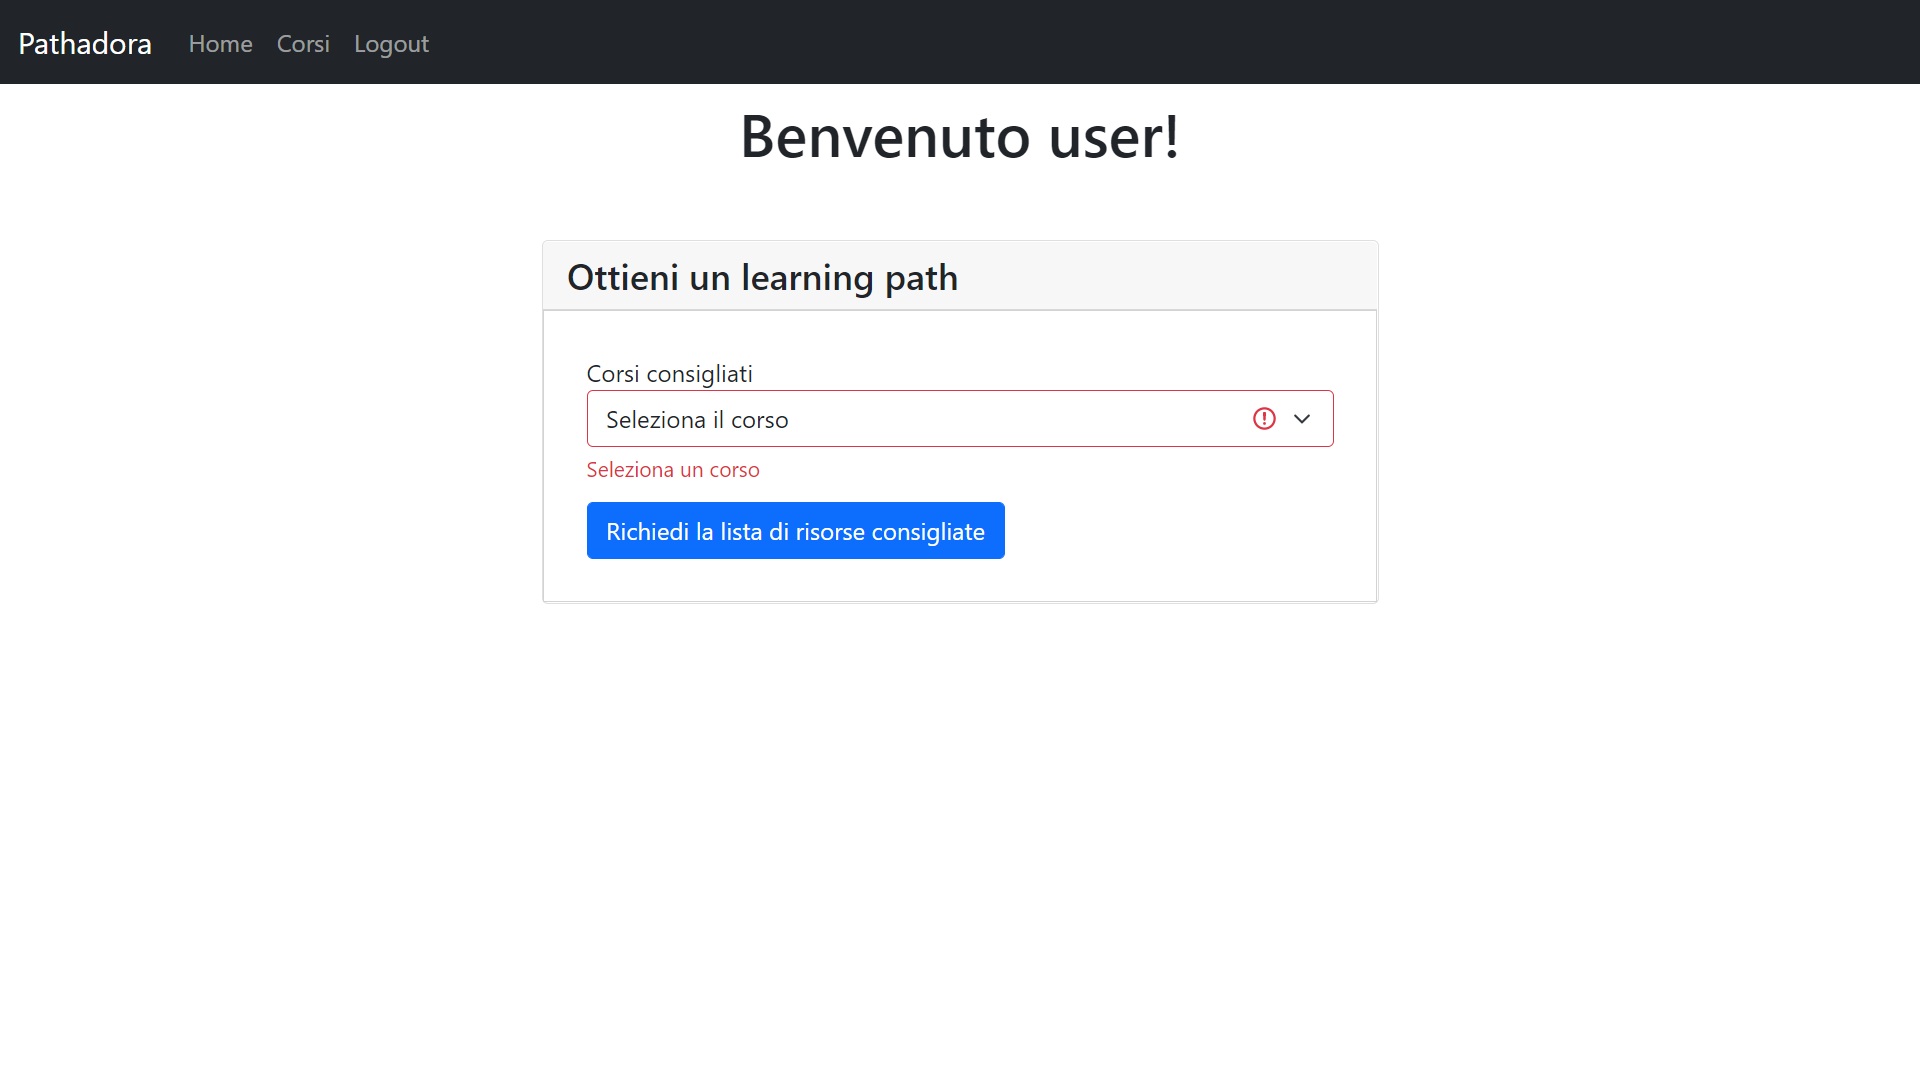
\includegraphics[scale=0.4]{res/resources-generation.png}
\caption{Form di richiesta risorse suggerite}
\label{fig:resources-generation}
\end{figure}

\begin{figure}[H]
\centering
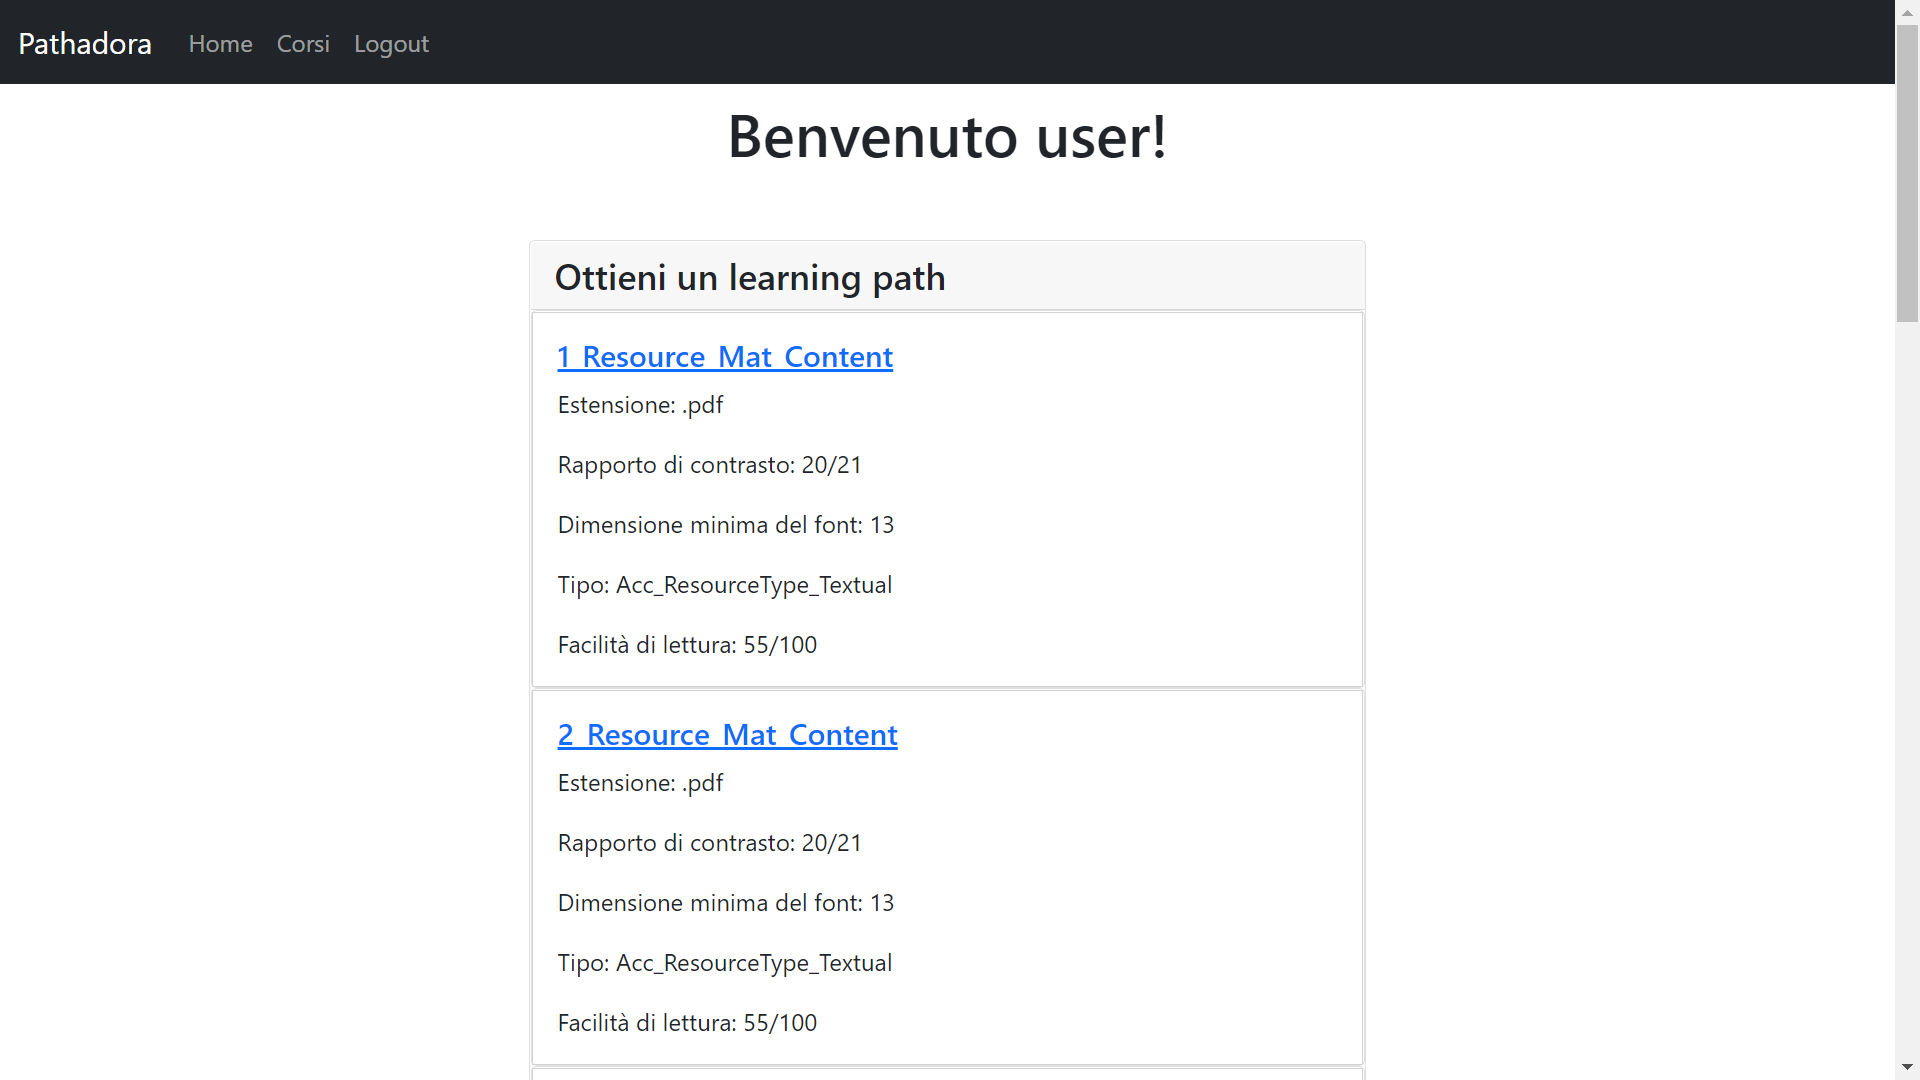
\includegraphics[scale=0.4]{res/path-result.png}
\caption{Risultato risorse suggerite}
\label{fig:resources-generation}
\end{figure}

\subsection{Ontologia}
L’ontologia pathadora-ontology racchiude tutti i concetti del sistema, importando altre ontologie pubbliche come LOM e AccessibleOCW, in modo da offrire un modello completo per la rappresentazione della conoscenza.

\subsubsection{Learner}
L'entità \texttt{Learner} modellata in Pathadora è lo stesso concetto rappresentato nell'ontologia \texttt{AccessibleOCW}. A tale entità vengono aggiunte altre proprietà per definire semanticamente le sue caratteristiche.

Tramite la proprietà \texttt{hasDegree}, l'ontologia permette di modellare i diplomi conferiti dallo studente. La proprietà \texttt{futureDegree} mette in relazione lo studente con il tipo di diploma che vorrebbe conferire nel futuro. Tramite \texttt{hasGoals}, l'ontologia modella gli obbiettivi dello studente e fornisce anche delle sottoproprietà basandosi sul tipo dell'obbiettivo (ad esempio \texttt{isPathDriven}, \texttt{isScoreDriven}, \texttt{isTimeDriven}, etc). Lo stile d'apprendimento di uno studente viene specificato tramite la proprietà \texttt{learningStyle}. Come nel caso degli obbiettivi, anche le passioni vengono modellate tramite la proprietà \texttt{passionateOf} e le sottoproprietà in base alla tipo della passione. Le informazioni che riguardano le lingue che uno studente potrebbe parare vengono inserite tramite la proprietà \texttt{speaks}.
La proprietà \texttt{hasDisability} rappresenta le informazioni che riguardano le disabilità dello studente e come range di valori aspetta un istanza della classe \texttt{Disabilities}.

\subsubsection{University}
L'organizzazione di tale istituzione viene rappresentata tramite una gerarchia di classi. I dipartimenti associati ad una scuola vengono messi in relazione tramite la proprietà \texttt{departmentOf}, mentre le facoltà di un dipartimento vengono specificate tramite \texttt{facultyOfDepartment}. Seguendo la stessa logica, i corsi vengono associati ad una facoltà tramite la proprietà \texttt{courseOfFaculty}. La proprietà \texttt{courseLanguage} permette di specificare in quale lingue verranno tenute le lezione di un corso. Un determinato corso viene dichiarato come obbligatorio oppure opzionale tramite la proprietà \texttt{isCourseObligatory} avendo come range un tipo di dato \texttt{boolean}. Le proprietà \texttt{courseSSD} e \texttt{courseType} mettono in relazione rispettivamente un corso con il suo tipo e il suo settore scientifico. Il range di queste due proprietà deve essere un istanza delle classi \texttt{CourseSSD} e \texttt{CourseType}. 

Per le istanze che rappresentano i corsi, sono state definite un insieme di proprietà dei dati tra le quali:
\begin{itemize}
    \item \texttt{coursePeriod}: specifica il periodo del corso;
    \item \texttt{courseCFU}: specifica i CFU del corso;
    \item \texttt{courseYear}: specifica l'anno del corso;
\end{itemize}

\subsubsection{LearningObject}
Nella spiegazione delle ontologie \texttt{LOM} e \texttt{AccessibleOCW}, abbiamo visto la modellazione delle risorsa da due punti di vista diversi basandosi sui metadati e sull'accessibilità. Pathadora tende di sincronizzare questi due punti di vista, aggiungendo nuovi concetti nella rappresentazione delle informazioni che riguardano le risorse.

Alla modellazioni \texttt{AccessibleOCW} vengono inserite delle proprietà che descrivono il livello dell'accessibilità, mappando la modalità d'accesso ad un risorsa con in tipo di dato numerico. Le tre proprietà da prendere in considerazione sono:
\begin{itemize}
    \item \texttt{resourceContrastRatio}: coefficiente che rappresenta il contrasto visivo della risorsa in un range da $\{1,...,100\}$;
    \item \texttt{resourceReadingEase}: coefficiente che specifica la leggibilità di una risorsa in base al numero di parole in una frase, la lunghezza del testo, in numero di sillabi, etc. Il range del coefficiente va da $\{1,...,100\}$;
    \item \texttt{resourceFontSize}: specifica la dimensione del font del testo e lo mappa in un coefficiente d'accessibilità;
\end{itemize}

L'ontologia tramite la proprietà \texttt{resourceType} associa ad una risorsa un il tipo che potrebbe essere testuale, video, audio, immagine, etc. Tutti gli elementi sviluppati nelle ontologie \texttt{LOM} e \texttt{AccessibleOCW} vengono utilizzati per specificare le caratteristiche delle risorse.

\subsubsection{Disabilities}
Pathadora si basa principalmente sull'ontologia \texttt{AccessibleOCW} per modellare le disabilità di uno studente, però aggiunge delle proprietà non gestite da tale ontologia. Pathadora definisce un insieme  di proprietà dei dati per rappresentare il livello d'accessibilità di uno studente, ad esempio \texttt{autismSpectrumLevel}, \texttt{blindnessLevel}, \texttt{hearingLossLevel}, etc). Durante la registrazione l'utente dovrebbe specificare questi livelli, anche stimarli in modo non preciso, per permettere al sistema di interpretali e mapparli con i coefficienti d'accessibilità delle risorse.

La proprietà \texttt{hasDisabilites} mette in relazione uno studente con un tipo di disabilità. Pathadora raggruppa le disabilità in diverse categorie che saranno istanze delle classi \texttt{Intellectual}, \texttt{Physical} e \texttt{Sensory}.